\documentclass[10pt, a4paper]{article}
\usepackage{geometry}
\geometry{a4paper,total={6in, 8in}, margin=0.25in}
\usepackage{booktabs}
\usepackage{amssymb}
\usepackage{graphicx}
\DeclareGraphicsExtensions{.png}

\newcommand\showdiv[1]{\overline{\smash{\hstretch{.5}{)}\mkern-3.2mu\hstretch{.5}{)}}#1}}
\newcommand\ph[1]{\textcolor{white}{#1}}

\begin{document}

\begin{enumerate}
\item\mbox{}
    \begin{enumerate}
    \item\mbox{}\\
        $\frac{600 \times 10^6 / 2}{2 \times 10^6} = 150$
    \item\mbox{}\\
        If the packet size is too big, the data the server need to manage would exceed the server's I/O bus speed threshold. The limitation can be shown as:\\
        $1000 \times \mbox{PS} \leq 600 \times 10^6 / 2$\\
        $\Rightarrow PS \leq 300 \times 10^3 (bit) = 37.5 (KB)$\\
        where PS is packet size\\
        throughput $ = f(PS) = \left\{
            \begin{array}{ll}
                1000 \mbox{PS} & \mbox{when PS} \leq 37.5 (KB)\\
                300 \times 10^6 & \mbox{when PS} > 37.5 (KB)
            \end{array}
        \right.$
    \item\mbox{}\\
        The limiting factor is not memory bandwidth but I/O bus speed.\\
        From (b), the I/O bus speed will become the limiting factor when the packet size exceed $37.5 (KB)$
    \end{enumerate}

\item\mbox{}
    \begin{enumerate}
    \item\mbox{}\\
        S1\\
        \begin{tabular}{cccc}
            \toprule
            Port IN & VCI IN & Port OUT & VCI OUT\\
            \hline
            1 & 0 & 3 & 0\\
            1 & 1 & 3 & 1\\
            3 & 0 & 0 & 0\\
            3 & 1 & 0 & 1\\
            2 & 0 & 3 & 2\\
            \bottomrule
        \end{tabular}\\

        S2\\
        \begin{tabular}{cccc}
            \toprule
            Port IN & VCI IN & Port OUT & VCI OUT\\
            \hline
            1 & 0 & 0 & 0\\
            1 & 1 & 2 & 0\\
            3 & 0 & 1 & 0\\
            0 & 0 & 1 & 1\\
            1 & 2 & 3 & 0\\
            \bottomrule
        \end{tabular}\\

        S3\\
        \begin{tabular}{cccc}
            \toprule
            Port IN & VCI IN & Port OUT & VCI OUT\\
            \hline
            3 & 0 & 1 & 0\\
            2 & 0 & 3 & 0\\
            1 & 0 & 2 & 0\\
            \bottomrule
        \end{tabular}\\

        S4\\
        \begin{tabular}{cccc}
            \toprule
            Port IN & VCI IN & Port OUT & VCI OUT\\
            \hline
            2 & 0 & 0 & 0\\
            2 & 1 & 3 & 0\\
            \bottomrule
        \end{tabular}
    \item\mbox{}\\
        \begin{tabular}{l|cccc}
            & Port 0 & Port 1 & Port 2 & Port 3\\
            \hline
            S1 & 2 & 0 & 0 & 3\\
            S2 & 1 & 2 & 1 & 1\\
            S3 & 0 & 1 & 1 & 1\\
            S4 & 1 & 0 & 0 & 1
        \end{tabular}
    \item\mbox{}\\
        0\ 0\ 0\ 0\ 0
    \item\mbox{}\\
        0\ 2\ 0\ 0
    \end{enumerate}

\item\mbox{}
    \begin{enumerate}
    \item\mbox{}\\
        The root bridge is B1.\\
        \begin{tabular}{cc}
            \toprule
            LAN & Designated Bridge\\
            \hline
            A & B5\\
            B & B4\\
            C & B9\\
            D & B3\\
            E & B1\\
            F & B8\\
            G & B1\\
            \bottomrule
        \end{tabular}
        \qquad
        \begin{tabular}{cc}
            \toprule
            Bridge & Root Port\\
            \hline
            B1 & -\\
            B2 & -\\
            B3 & A\\
            B4 & G\\
            B5 & E\\
            B6 & -\\
            B7 & -\\
            B8 & E\\
            B9 & F\\
            \bottomrule
        \end{tabular}
    \item\mbox{}\\
        \begin{tabular}{lll}
            \toprule
            Source & Destination & LANs the message is heard on\\
            \hline
            Mars & Venus & ABCDEFG\\
            Venus & Mars & BG\\
            Jupiter & Venus & ACDEFG\\
            \bottomrule
        \end{tabular}
    \end{enumerate}

\item\mbox{}
    \begin{enumerate}
    \item\mbox{}\\
        $\frac{1800}{2 \times 10^8} + 5 \times \frac{20}{50 \times 10^6} = 11 \times 10^{-6} (s) = 11 (\mu s)$
    \item\mbox{}\\
        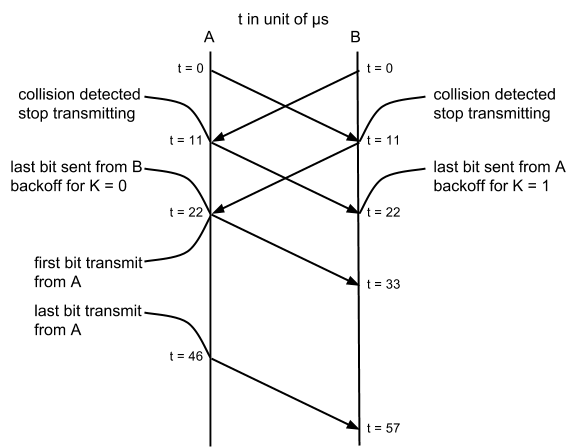
\includegraphics[height=3in]{images/problem_4b}\\
        At time $t = 11 (\mu s)$, both A and B detect an collision, so both A and B stop transmitting at time $t = 11 (\mu s)$. At time $t = 22 (\mu s)$, the last bit from the other side reached, and A backoffs for $K = 0$, B backoffs for $K = 1$, which denotes $\frac{1000 \times 1}{50 \times 10^6} = 20 \times 10^{-6} (s) = 20 (\mu s)$. However, before B starts to retransmit, the first bit retransmitted by A already arrives B at $t = 22 + 11 = 33 (\mu s) < 22 + 20 = 42 (\mu s)$. Therefore, B will backoff again till the transmission from A completes.\\
        Finally, the time that A's packet is completely delivered to B is\\
        $33 \times 10^{-6} + \frac{150 \times 8}{50 \times 10^6} = 57 \times 10^{-6} (s)$\\
        $= 57 (\mu s)$
    \item\mbox{}\\
        $11 \times 10^{-6} + \frac{150 \times 8}{50 \times 10^6} \times 6 + \frac{20}{50 \times 10^6} \times 5 = 155 \times 10^{-6}$\\
        $155 (\mu s)$
    \end{enumerate}

\item\mbox{}
    \begin{enumerate}
    \item\mbox{}\\
        Because A needs to transmit for $\frac{1024}{20 \times 10^6} = 51.2 \times 10^{-6} (s) = 51.2 (\mu s)$, and the first bit transmitted from B is detected by A at time $t = 15 \times 10^{-6} \times 2 = 30 \times 10^{-6} (s) = 30 (\mu s)$. Therefore, A does not finish transmitting the frame before it detects that there was a collision.
    \item\mbox{}\\
        At time $t = 30 (\mu s)$, A detects a collision, and the time A needs to transmit preamble is $\frac{128}{20 \times 10^6} = 6.4 \times 10^{-6} (s) = 6.4 (\mu s)$, which is less than $30 (\mu s)$. Therefore, we conclude that A just need to send a jamming sigmal right after the collision.\\
        The time A finish sending a jamming signal is:\\
        $30 \times 10^{-6} + \frac{64}{20 \times 10^6} = 33.2 \times 10^{-6} (s)$\\
        $= 33.2 (\mu s)$\\
        At time $t = 15 (\mu s)$, B detects a collision, and B has not transmitted any data yet. Therefore, B needs to transmit the preamble before the jamming signal.\\
        The time B finish sending a jamming signal is:\\
        $15 \times 10^{-6} + \frac{128 + 64}{20 \times 10^6} = 24.6 \times 10^{-6} (s)$\\
        $= 24.6 (\mu s)$
    \item\mbox{}\\
        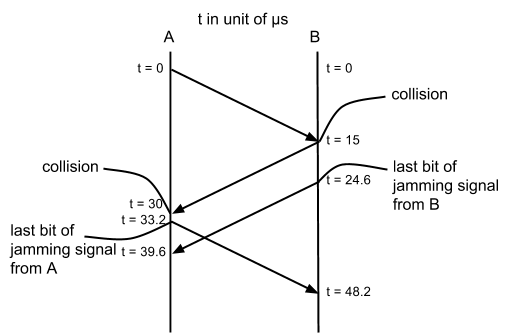
\includegraphics[height=2.5in]{images/problem_5c}\\
        B sends the last bit of the jamming signal at time $t = 24.6 (\mu s)$, so the jamming signal sent from B will arrive A at time $t = 24.6 + 15 = 39.6 (\mu s)$. Therefore, the time A first hear an idle channel is at $t = 39.6 (\mu s)$.\\
        A sends the last bit of the jamming signal at time $t = 33.2 (\mu s)$, so the jamming signal sent from A will arrive B at time $t = 33.2 + 15 = 48.2 (\mu s)$. Therefore, the time B first hear an idle channel is at $t = 48.2 (\mu s)$.
    \item\mbox{}\\
        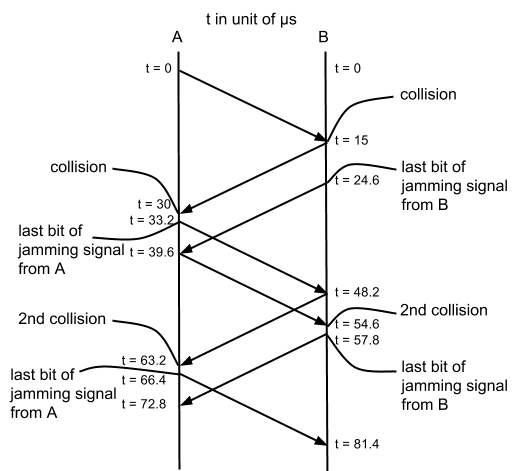
\includegraphics[height=3.5in]{images/problem_5d}\\
        B detects the second collision at time $t = 39.6 + 15 = 54.6 (\mu s)$, and the time the last bit sent from B is $t = 54.6 \times 10^{-6} + \frac{64}{20 \times 10^6} = 57.8 \times 10^{-6} (s) = 57.8 (\mu s)$. Therefore, the last bit will arrive A at time $t = 57.8 + 15 = 72.8 (\mu s)$.\\
        A will next hear the idle channel at $t = 72.8 (\mu s)$\\
        A detects the second collision at time $t = 48.2 + 15 = 63.2 (\mu s)$, and the time the last bit sent from A is $t = 63.2 \times 10^{-6} + \frac{64}{20 \times 10^6} = 66.4 \times 10^{-6} (s) = 66.4 (\mu s)$. Therefore, the last bit will arrive A at time $t = 66.4 + 15 = 81.4 (\mu s)$.\\
        A will next hear the idle channel at $t = 81.4 (\mu s)$
    \item\mbox{}
    \end{enumerate}
        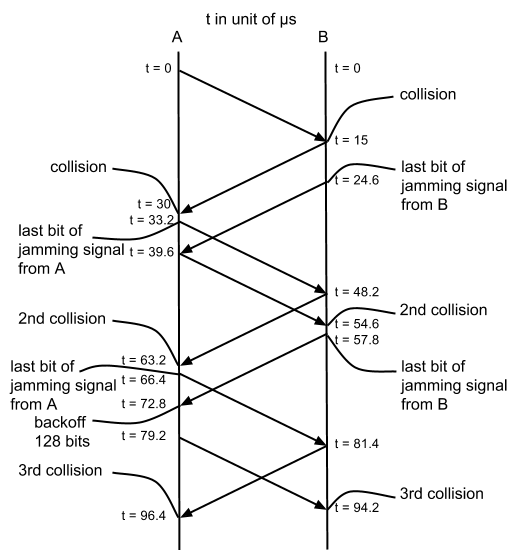
\includegraphics[height=4in]{images/problem_5e}\\
        The idle time occurs after the second collision at B is $t = 81.4 (\mu s)$, and the idle time occurs after the second collision at A is $t = 72.8 (\mu s)$. Therefore, the message from B will arrive A at time $t = 81.4 + 15 = 96.4 (\mu s)$, and A will try to retransmit at time $t = 72.8 \times 10^{-6} + \frac{128}{20 \times 10^6} = 79.2 \times 10^{-6} (s) = 79.2 (\mu s)$. In addition, A needs to transmit for $\frac{1024}{20 \times 10^6} = 51.2 \times 10^{-6} (s) = 51.2 (\mu s)$.\\
        $\because 79.2 + 51.2 = 130.4 > 96.4$\\
        $\therefore$ The transmission of host B is unsuccessful

\item\mbox{}\\
    \begin{tabular}{cll}
        \toprule
        Step & Confirmed & Relative\\
        \hline
        1 & (A, 0, -) & \\
        2 & (A, 0, -) & (B, 1, B), (C, 7, C)\\
        3 & (A, 0, -), (B, 1, B) & (C, 7, C)\\
        4 & (A, 0, -), (B, 1, B) & (C, 7, C), (E, 4, B), (D, 6, B)\\
        5 & (A, 0, -), (B, 1, B), (E, 4, B) & (C, 7, C), (D, 6, B)\\
        6 & (A, 0, -), (B, 1, B), (E, 4, B) & (C, 7, C), (D, 5, B), (F, 13, B)\\
        7 & (A, 0, -), (B, 1, B), (E, 4, B), (D, 5, B) & (C, 7, C), (F, 13, B)\\
        8 & (A, 0, -), (B, 1, B), (E, 4, B), (D, 5, B) & (C, 7, C), (F, 6, B)\\
        9 & (A, 0, -), (B, 1, B), (E, 4, B), (D, 5, B), (F, 6, B) & (C, 7, C)\\
        10 & (A, 0, -), (B, 1, B), (E, 4, B), (D, 5, B), (F, 6, B) & (C, 7, C)\\
        11 & (A, 0, -), (B, 1, B), (E, 4, B), (D, 5, B), (F, 6, B), (C, 7, C) & \\
        \bottomrule
    \end{tabular}
\end{enumerate}

\end{document}
